\documentclass[a4papper]{article}
\usepackage[utf8]{inputenc}
\usepackage[14pt]{extsizes}
\usepackage[english,russian]{babel}
\usepackage{amsmath}
\usepackage{amsfonts}
\usepackage{graphicx}
\usepackage{algorithm}
\usepackage{algpseudocode}
\usepackage[left=20mm, top=15mm, right=15mm, bottom=15mm, nohead, footskip=10mm]{geometry}

\newcommand{\angstrom}{\text\normalfont\AA}
\newcommand{\bb}{\textbf}
\newcommand{\ls}{\left[}
\newcommand{\rs}{\right]}
\newcommand{\lp}{\left(}
\newcommand{\rp}{\right)}
\newcommand{\la}{\leftarrow}
\newcommand{\eps}{\varepsilon}

\begin{document}
\begin{titlepage}
\begin{center}
    \large
    \textbf{МИНИСТЕРСТВО ОБРАЗОВАНИЯ РЕСПУБЛИКИ БЕЛАРУСЬ}
    \vspace{0.25cm}

    \textbf{БЕЛОРУССКИЙ ГОСУДАРСТВЕННЫЙ УНИВЕРСИТЕТ}
    \vspace{0.25cm}

    \textbf{ФАКУЛЬТЕТ ПРИКЛАДНОЙ МАТЕМАТИКИ И ИНФОРМАТИКИ}

    \textbf{Кафедра биомедицинской информатики}
    \vfill


    \textbf{Тема курсовой}
    \vfill

    Курсовая работа

\end{center}
\vfill

\newlength{\ML}
\hfill\begin{minipage}{0.45\textwidth}
    Рака Алексей Степановича\\
    студента 3 курса,\\
    специальность <<Информатика>>
    \vspace{0.25cm}

    Научный руководитель:\\
    Хадарович А.Ю.
\end{minipage}
\bigskip


\begin{center}
    Минск, 2018
\end{center}

\end{titlepage}
\section{ Введение }
Выравнивание структуры белка – это ценный инструмент для фолдинга белков и классифицикации функций. Успех структурной геномики, направленной на экспериментальное определение трёхмерных структур тысяч репрезентативных белков, в решающей степени зависит от нашей способности разрабатывать точные инструменты для сравнения белковых структрур. Однако, несмотря на свою исключительную важность, проблема по-прежнему не имеет быстрого и точного решения. В то время, как некоторые функции скоринга структурного полобия могут быть аппроксимированы за полиномиальное время, нат никакой процедуры для оптимизации любой меры структурного выравнивания. В своей обзорной статье о прогрессе в области сравнения структур Тейлор и коллеги пишут: “в сравнении структур у нас даже нет алгоритма, который гарантирует оптимальный овтет для пары структур”.

Существует несколько различных, но связанных между собой определений оптимального выравнивания двух белков. Некоторые методы определяют оптимальную суперпозицию, минимизирующую расстояние между выровненными атомами. Другие методы пытаются минимизировать разницу между внутриатомными расстояниями.

Недавно было введено несколько методов улучшения соответствия белковых структур, включая методы, основанные на фенотипической пластичности и метод гибких выравниваний последовательностью локальных преобразований.

Пожалуй, наиболее интуитвиной и широко используемой мерой подобия двух белков является наибольшее количество атомов в двух структурах, которые могут быть совмещены друг с другом на заданное расстояние. Далее будем обозначать эту метрицу $CA \leq \sigma$, где $\sigma > 0$ обозначает порог расстояния в ангстремах.

Многие меры структурного выравнивая построены на $CA \leq \sigma$, включая GDT, AL0, MaxSub, CA-atoms < 3\angstrom, Q-score и TM-score. Global Distance Test (GDT) обычно используется для оценки качества моделей в эксперименте CASP. Точность прогнозируемой модели в CASP измеряется оценкой GDT\_TS, которая представляет собой среднее значение оценок GDT, вычисленных на нескольких порогах расстояния. Точнее,
\begin{gather*}
\mathrm{GDT\_TS} = \frac{(\mathrm{GDT\_P1} + \mathrm{GDT\_P2} + \mathrm{GDT\_P4} + \mathrm{GDT\_P8})}{4}
\end{gather*}
Где $\mathrm{GDT\_Pn}$ определяет часть атомов CA, которые могут быть совмещены на расстоянии не превосходящем n ангстремов.

Одной из главных мер качества модели в LiveBench является CA-atoms < 3 \angstrom (в наших обозначениях CA < 3). Из-за сложности оптимизации самой функции подсчёта очков LiveBench приближается к CA < 3 с помощью 3deval, программы, которая пытается максимизировать другую метрицу, а именно 3D-оценку.

CAFASP бенчмарк использует MsxSub для оценки качества прогнозов. MaxSub определяется как взвешенная доля остатков в модели, попадающих в пределы 3.5 \angstrom от выровненных остатков в экспериментальной структуре.

Независимо от используемой системы подсчёта очков, основная трудность, которую должен преодолеть любой метод структурного выравнивания, -- это бесконечное (несчётное) пространство всех возможных структурных суперпозиций. Чтобы обойти эту проблему, текущие исследования в жтой области фокусируются науменьшении размера пространства поиска путём перечисления относительно небольшого, но репрезентативного набора суперпозиций. Однако, хотя решения, полученные эвристическими подходами, частично точны, они никогда не гарантируются даже близкими к оптимальным решениями.

Очевидным способом устранения ограничений эвристических методов является разработка быстрого и точного метода максимизации $CA \leq \sigma$. Такой метод позволил бы точно вычислить ряд мер структруного выравнивания, включая GDT\_TS, AL0 и MaxSum.

В данной работе рассмотрим алгоритм, который способен найти суперпозицию, которая достаточно близка к оптимальной суперпозиции. Более конкретно, для любого заданного расстояния среза $\sigma > 0$ и любого $\eps > 0$ алгоритм возвращает суперпозицию, которая помещает по крайней мере столько пар остатков на расстоянии не превосходящем $\sigma + \eps$ сколько оптимальная суперпозиция содержит пар на расстоянии не превосходящем $\sigma$. В дополнение к относительно низкой временной сложности и способности к параллельным реализациям, данный алгоритм обеспечивает "качество решения", которое определяется как разница между оценкой возвращённой суперпозиции и оценкой оптимальной суперпозиции. Метрика качества решения может использоваться для определения того, является ли возвращённая суперпозиция оптимальной суперпозицией (или необходим дургой более подробный поиск).

Данный алгоритм приближённого решения основан на схеме Колодного и Линиала для аппроксимации для класса непрерывных мер структурного подобия, работающей за полиномиальное время. Однако представленные здесь  результаты не могут быть получены из их исследования, поскльку целевая функция $CA \leq \sigma$ не относится к категории оценочных функций описываемых Колодным и Линиалом функций. На самом деле, класс оценочных функций поддающихся методам Колодного и Линиала (а именно в классу функций удовлетворяющих условию Липшица) не включает в себя GDT\_TS, AL0, MaxSum, TM-score, Q-score и некоторые другие меры структурного сходства белков.

Наконец, в данной работе решается проблема нахождения процедуры, которая возвращает опптимальную суперпозицию двух структур. Здесь представляется процедура, которая гарантированно вернёт оптимальное решение с вероятностью 1, т.е. для всех, кроме конечного значений, расстояний. Однако подчеркнём, что алгорим оптимального решения не работает за полиномиальное время. Так же известно, что это проблема является NP-трудной.

\section{ Методы и результаты }
\subsection{Предварительные сведения и определения}

Задача выравнивания структуры пары белков может быть сформулирована следующим образом: "Учитывая два белка a и b и расстояние среза $\sigma > 0$, найти жёсткое преобразование $t$ и соответствие остаток-остаток (выравнивание), которое максимизирует количество пар остатков $a$ и $t(b)$ на расстоянии $\leq \sigma$". Мы назваыаем $t$ -- $\sigma$-оптимальное преобразование для $a$ и $b$. Отметим, что, не теряя общности, можно предположить, что белок $a$ удерживается фиксированным, в то время как белок $b$ трансформируется.

Для того, чттобы точно сормулировать вышеуказанную проблему, нам нужны некоторые определения.

\bb{Определение} Белок -- это последовательность точек в трёхмерном пространстве:
\begin{gather*}
a = (a_1, a_2, \dots, a_n), a_i \in \mathbb{R}^3, i = \overline{1, n}
\end{gather*}
Во многих приложениях, $ a_i$ представляет собой CA-остаток.

\bb{Определение} Выравнивание белков $a = (a_1, a_2, \dots, a_n)$ и $b = (b_1, b_2, \dots, b_m)$ -- это последовательность пар точек из $a$ и $b$:
\begin{gather*}
S(a, b) = ((a_{i_1}, b_{j_1}), \dots, (a_{i_k}, b_{j_k}))
\end{gather*}
где $1 \leq i_1 < \dots < i_k \leq n$ и $1 \leq j_1 < \dots < j_k \leq m$.

\bb{Определение} $\sigma$-оптимальное выравнивание белков $a = (a_2, a_2, \dots, a_n)$ и $b = (b_1, b_2, \dots, b_m)$, обозначается $S(a, b, \sigma)$ это выравниванеи $a$ и $b$, которое максимизирует число выровненных точек $a$ и $b$ на расстоянии $\sigma$.

В приведённом выше определении мы предполагаем, что белки $a$ и $b$ зафиксированы в пространстве. $S(a, b, \sigma )$ относятся к оптимальному спариванию аминокислотных букв буще изменения структурной суперпозиции. Хорошо известно, что для любых двух фиксированных в пространстве белков $a$ и $b$ длины $n$ и любого $\sigma > 0$  выравнивание $S(a, b, \sigma )$ может быть вычислено за время $O(n^2)$ с использованием динамического программирования. Теперь мыбудет использовать $|S(a, b, \sigma )|$ для обозначения количества пар точек в $S(a, b, \sigma )$ на расстоянии $\leq \sigma$

\bb{Определение} $\sigma$-оптимальная трансформация для $a$ и $b$, обозначается $t^\sigma$, -- это жёсткая трансформация, которая максимизирует $|S(a, t(b), \sigma)|$ в множестве всех жёстких трансформаций. Другими словами:
\begin{gather*}
t^\sigma = \arg \max_t |S(a, t(b), \sigma)|
\end{gather*}
Легко увидеть, что CA $\leq \sigma$ в точность $|S(a, t^\sigma (b), \sigma)|$, где $t^\sigma$ -- это $\sigma$-оптимальная трансформация $a$ и $b$.

\bb{Определение} Трансформация $t$ удовлетворяет:
\begin{gather*}
|S(a, t(b), \sigma + \eps)| \geq |S(a, t^\sigma (b), \sigma)|
\end{gather*}
Это называется $(\sigma, \eps)$-трансформация $a$ и $b$, обозначается $t_\eps^\sigma$.

Нужно отметить, что $t_\eps^\sigma$ -- это любая трансформация $t$ с таким свойством, что пары точек в структурах $a$ и $t(b)$, которые могут быть совмещены на расстоянии $\leq \sigma + \eps$ не меньше, чем количество таких пар в структурах $a$ и $t^\sigma(b)$.

Так же напомним, что любая ориентация, сохраняющая жёсткое преобразование $t$ является композицие вращения и переноса $t = t_{tr} \circ t_{rot}$. Любая такая трансформация может быть представлена как точка в шестимерном пространстве:
\begin{gather*}
t = (\alpha, \beta, \gamma, u, v, w) \in \mathbb{R}^6
\end{gather*}
где $\alpha$ и $\gamma$ -- угла поворота вдоль оси $z$, $\beta$ -- это поворот вдоль оси $x$. а также $u, v, w$  -- это перенос вдоль оси $x, y, z$.

\subsection{ Почти оптимальное решение }
Без потери общности можно предположить, что оба белка $a$ и $b$ имеют центр масс в начале. Таким образом, суперпозиция, выравнивающая центр масс белков $a$ и $b$, будет первой (среди многих) суперпозиций, проверенной данным методом. Рассматриваемый алгоритм нахождения $t_\eps^\sigma$, называемый $\eps$-оптимальным, основан на непрерывности жёстких преобразований. Другими словами, небольшое изменение любого из шести аргументов $T=(\alpha, \beta, \gamma, u, v, w)$ приводит к небольшому изменению пространственного положения белка $B$. Например, если $b$ вращается вокруг оси $x$ на небольшой угол $\delta > 0$, то расстояние пройденное любой точкой $p(x, y, z) \in b$ будет равно:
\begin{gather*}
d = \sqrt{2(y^2 + z^2)(1 - \cos \delta)} \leq \sqrt{2}R_b\sin\delta \leq \sqrt{2} R_b\delta
\end{gather*}  
где $R_b$ -- это радиус минимальной сферы содержащей в себе $b$.

\subsection{ Алгоритма нахождения почти оптимального решения}

Несложно увидеть, что кандидатами для $t_\eps^\sigma$ являются только те преобразование, которые не удаляют белок $b$ далеко от $a$, т.е. преобразования $t=(\alpha, \beta, \gamma, u, v, w) \in \mathbb{R}^6$ из замкнутого интервала:
\begin{gather*}
I = [0, 2\pi] \times [0, \pi] \times [0, 2\pi] \times [-M_x, M_x] \times [-M_y, M_y] \times [-M_z, M_z]
\end{gather*}
где
\begin{gather*}
M_x = \frac{m_x^a + m_x^b}{2}, M_y = \frac{m_y^a + m_y^a}{2}, M_z = \frac{m_z^a + m_z^b}{2}
\end{gather*}
и $m_x^a, m_y^a, m_z^a, m_x^b, m_y^b, m_z^b$ --размер наименьшего интервала $B(a)$ и $B(b)$ в $\mathbb{R}^3$ содержащие $a$ и $b$.\\
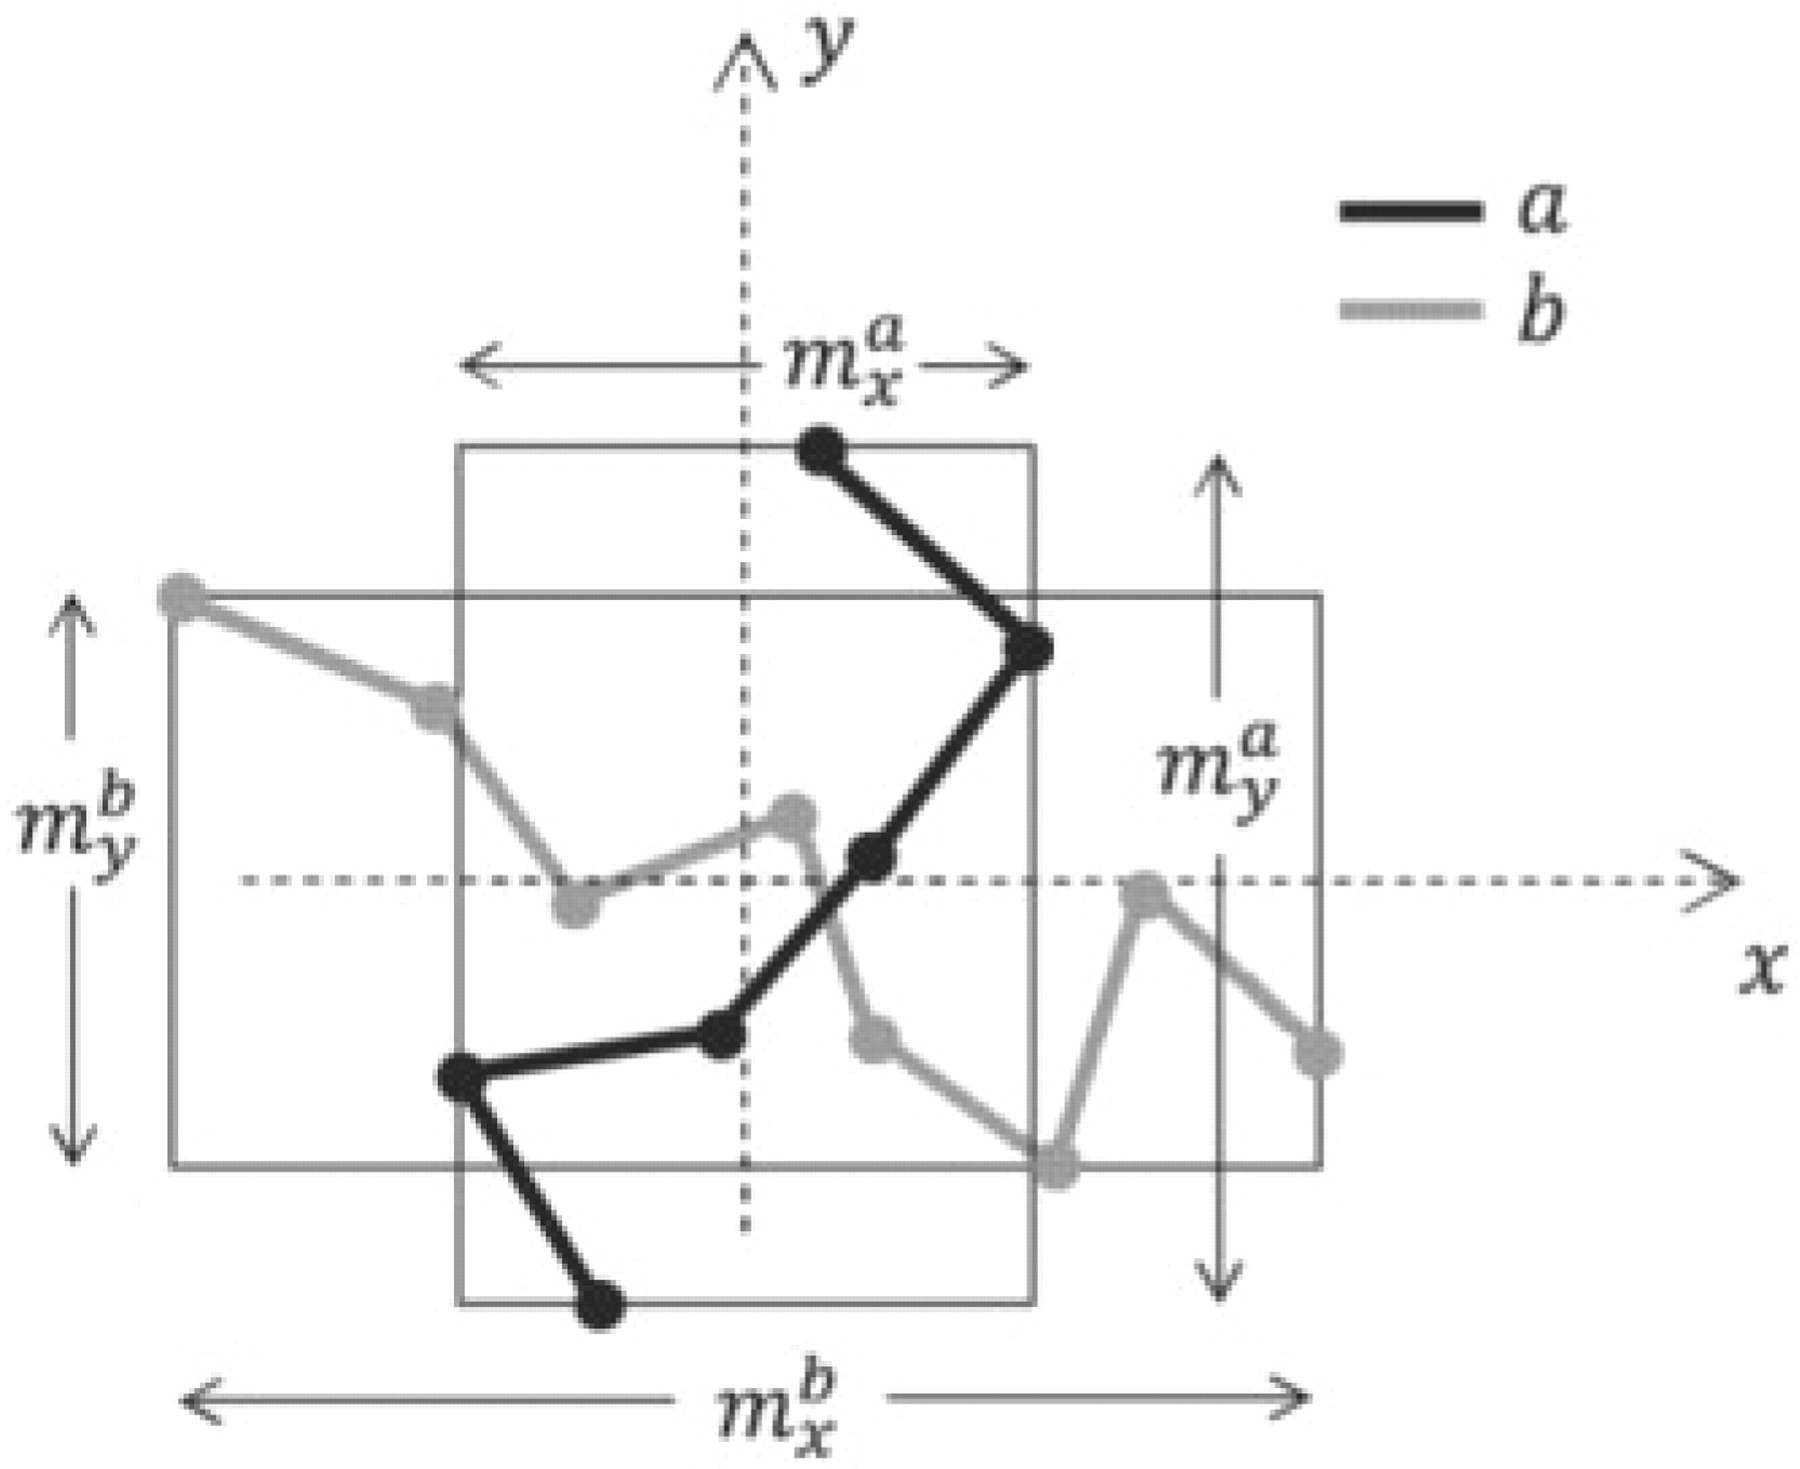
\includegraphics[scale=0.3]{../pictures/btp530f1.jpeg}\\
Для дальнейшего уменьшения размера пространства определим конечную $\eps$-сеть преобразований из интервала $I$, полученную разбиением на небольшие шестимерные ячейки. Точки $\eps$-сети являются вершинами этих ячеек.
\begin{gather}
d_1 = d_2 = d_3 = \frac{\eps}{3\sqrt{2}R_b}\\
d_4 = d_5 = d_6 = \frac{\eps}{\sqrt{3}}
\end{gather}
Заметим, что для нахождения $t_\eps^\sigma$ достаточно проверить преобразования из $\eps$-сети. Это происходит потому, что для каждого $t=(\alpha, \beta, \gamma, u, v, w) \in I$, суещствует такая формула преобразования, что:
\begin{gather}
|\alpha - \overline{\alpha}| \leq \frac{d_1}{2}, |\beta - \overline{\beta}| \leq \frac{d_2}{2}, |\gamma - \overline{\gamma}| \leq \frac{d_3}{2}\\
|u - \overline{u}| \leq \frac{d_4}{2}, |v - \overline{v}| \leq \frac{d_5}{2}, |w - \overline{w}| \leq \frac{d_6}{2}
\end{gather}
и следовательно
\begin{gather}
\| t(b_i) - \overline{t}(b_i)\| \leq \eps, \forall b_i \in b
\end{gather}
где $\| t(b_i) - \overline{t}(b_i)\| $ обозначает Евклидово расстояние между $t(b_i)$ и $\overline{t}(b_i)$. В частности, если $t$ -- это $\sigma$-оптимальное преобразование $t^\sigma$, тогда $\overline{t}$ -- это $(\sigma, \eps)$-оптимальное преобразование $t_\eps^\sigma$.

Псевдо-код данного алгоритма:
\begin{algorithmic}[1]
\item Перенесём центры масс белков $a$ и $b$ в начало координат.
\item Вычислим $M_x, M_y, M_z, R_b$.
\item $r_{\alpha, \gamma} \la \ls \frac{6\sqrt{2}\pi R_b}{\eps}\rs$
\item $r_{\beta} \la \ls \frac{3\sqrt{2}\pi R_b}{\eps}\rs$
\item $s_x \la \ls 1 + \frac{2\sqrt{3}M_x}{\eps} \rs$
\item $s_y \la \ls 1 + \frac{2\sqrt{3}M_y}{\eps} \rs$
\item $s_z \la \ls 1 + \frac{2\sqrt{3}M_z}{\eps} \rs$
\item $d_r \la \frac{\eps}{3\sqrt{2}R_b}$
\item $d_t \la \frac{\eps}{\sqrt{3}}$
\item $bestScore \la 0$
\For{$0 \leq i_1 \leq r_{\alpha, \gamma}, 0 \leq i_2 \leq r_{\beta}, 0 \leq i_3 \leq r_{\alpha, \gamma}$}
\For{$0 \leq i_4 \leq s_x, 0 \leq i_5 \leq s_y, 0 \leq i_6 \leq s_z$}
\State $t \la (i_1d_r, i_2d_r, i_3d_r, -M_x + i_4d_t, -M_y + i_5d_t, -M_z + i_6d_t)$
\If {$|S(a, t(b), \sigma + \eps)| > bestScore$}
    \State $bestScore \la |S(a, t(b), \sigma + \eps)|$
    \State $t_{best} \la t$
\EndIf
\EndFor
\EndFor
\State \Return $t_{best}$
\end{algorithmic}
\subsection{Время работы}
Для пары белков длины $n$, худший слушай работы данного алгоритма происходит, когда радиус ограничивающей сферы белка $b$ линеен относительно $n$, то есть $R_b = O(n)$. В этом случае общее число преобразований, проверенных данным алгоритмом, равно $\mathbf{NET}(\eps) = O \lp \frac{n^6}{\eps^6} \rp$. Для каждого такого преобразования оптимальное соответствие может быть вычислено с использованием процедуры динамического программирования $O(n^2)$, что приводит к наихудшему времени работы $O \lp \frac{n^8}{\epsilon^6} \rp$.

Однако общая стоимость данного алгоритма, как правило, лучше на практике, так как объём белка пропорцианально масштабируется с количество остатков. Например, если $b$ -- глобулярный белок, тогда $R_b = O(n^\frac{1}{3})$, и таким образом время работы данного алгоритма равно только $O\lp\frac{n^4}{\eps^6}\rp$.

Для сравнения алгоритм Колодного и Линеала для оптимизации класса оценочных функций, удовлетворяющих условию Липшица, равна $O \lp \frac{n^{10}}{\eps^6} \rp$ для глобулярных и $O \lp \frac{n^{12}}{\eps^6} \rp$ для неглобулярных белков.

\subsection{ Качество решение}
Качество решения $t_\eps^\sigma$ представленного $\eps$-оптимальным алгоритмом определяется как разность между оценкой оптимального решения $t^\sigma$ и оценкой $t_\eps^\sigma$:
\begin{gather}
Err(t_\eps^\sigma ) = |S(a, t^\sigma (b), \sigma) | - (S(a, t_\eps^\sigma (b), \sigma)|
\end{gather}
Пока $Err(t_\eps^\sigma)$ не может вычислен в пределах временного окна $\eps$-оптималбного алгоритма (так как не известен $t^\sigma$), верхняя граница $Err(t_\eps^\sigma)$:
\begin{gather}
MaxErr(t_\eps^\sigma ) = |S(a, t_\eps^\sigma (b), \sigma + \eps)| - |S(a, t_\eps^\sigma(b), \sigma)|
\end{gather}
Данное выражение может вычислено за счёт маленькой можификации $\eps$-оптимального алгоритма, без увеличения ассимптотической сложности.

\subsection{Оптимальное решение}
Процедура нахождения оптимального решения базируется на том наблюдении, что $f(\sigma) = |S(a, t^\sigma (b), \sigma)|$ это функция, которую можно разбить на некоторое конечное число значений $\sigma_1, \dots, \sigma_k$. Если $\sigma > 0$ -- некоторое действительное число отличное от $\sigma_i, \forall i \in [1, k]$, тогда для достаточно малого $\eps > 0$ получаем $f(\sigma + \eps) = f(\sigma - \eps)$.	
\begin{gather*}
f(\sigma + \eps) = |S(a, t^{\sigma + \eps}, \sigma + \eps)| \geq |S(a, t_\eps^\sigma (b), \sigma + \eps)| \geq\\ \geq
|S(a, t^\sigma (b), \sigma)| \geq |S(a, t^{\sigma - \eps}_\eps (b), \sigma)| \geq \\ \geq
|S(a, t^{\sigma - \eps (b)}, \sigma - \eps)| = f(\sigma - \eps)
\end{gather*}
Отсюда следует, что для каждого такого $\eps$ существует преобразование $t_\eps^{\sigma - \eps}$, которое является оптимальным.\\
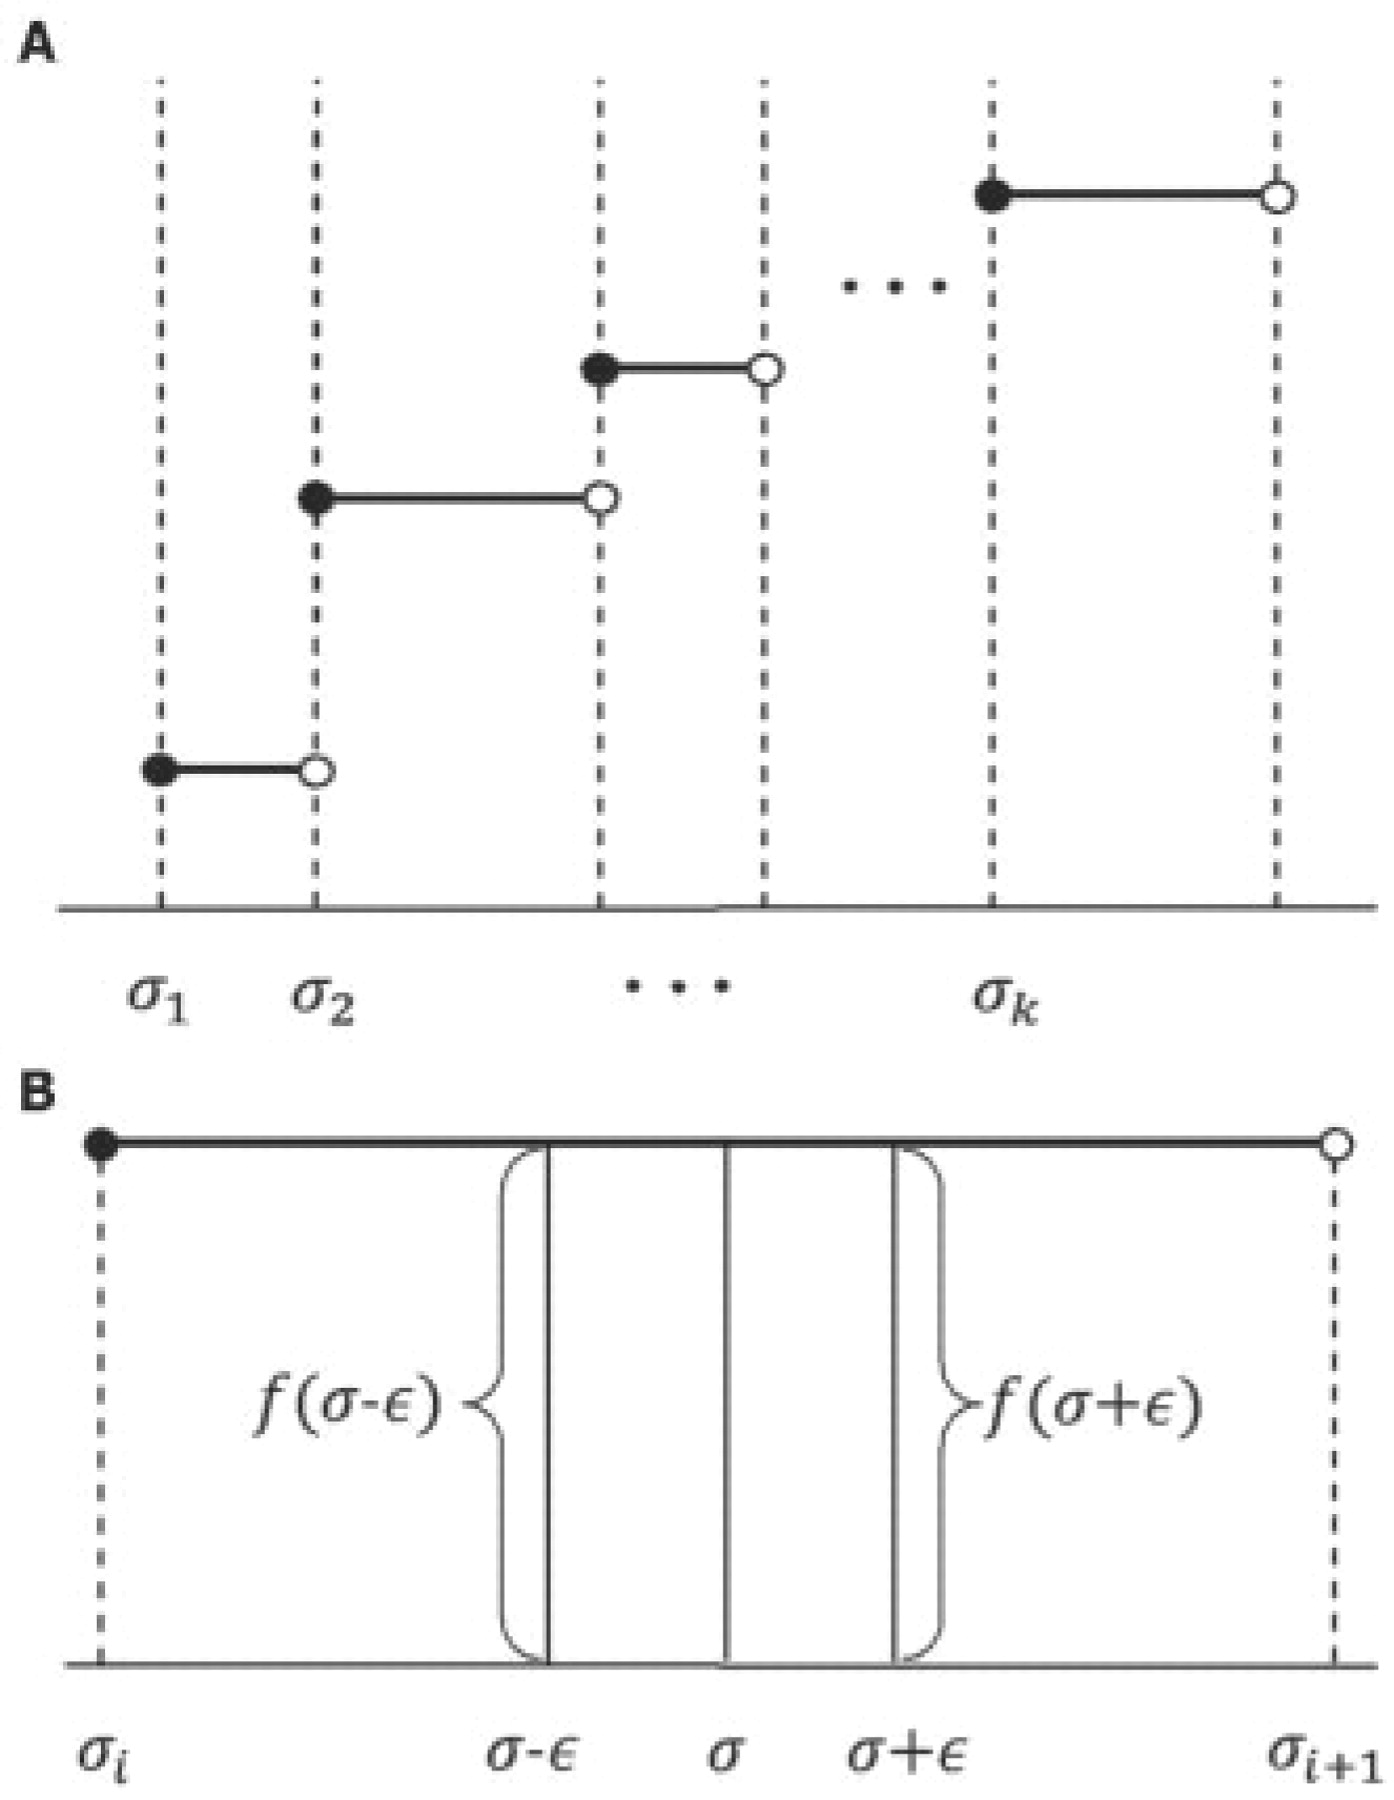
\includegraphics[scale=0.35]{../pictures/btp530f2.jpeg}\\
Опишем полученный алгоритм в виде псевдокода.

OPTIMAL($a, b, \sigma$). Отметим, что OPTIMAL возвращает оптимальное решение с вероятностью 1, то есть в случаях, когда $\sigma$ не совпадает ни с одним из фиксированных значений $\sigma_1, \dots, \sigma_k$. Однако число операций, выполненных OPTIMAL, ельзя оценить заранее, так как время её выполнения зависит от разности между $\sigma$ и ближайшим $\sigma_i$ (которая зависит от внутренней геометрии входных белков $a$ и $b$). 

\begin{algorithmic}[1]
\State $\eps \la 1$
\State $t_\eps^\sigma \la \mathrm{EPSILON-OPTIMAL}(a, b, \sigma, \eps)$
\State $t_eps^{\sigma - \eps} \la \mathrm{EPSILON-OPTIMAL}(a, b, \sigma - \eps, \eps)$
\State $\eps \la \frac{\eps}{2}$
\While{$|S(a, t_\eps^\sigma (b), \sigma + \eps )| - |S(a, t_\eps^{\sigma - \eps}(b), \sigma ) > 0$}
\State $t_\eps^\sigma \la \mathrm{EPSILON-OPTIMAL}(a, b, \sigma, \eps)$
\State $t_eps^{\sigma - \eps} \la \mathrm{EPSILON-OPTIMAL}(a, b, \sigma - \eps, \eps)$
\State $\eps \la \frac{\eps}{2}$
\EndWhile
\State \Return $t_\eps^{\sigma - \eps}$
\end{algorithmic}

\subsection{Практическое применение}
Помимо относительно малого времени работы, $\eps$-оптимальный алгортим поддаётся параллельным вычисления, так как NET ($\eps$) может быть разделена и процедура поиска будет проводиться одновременно на нескольких подмножествах NET($\eps$). Для оценки потенциальных преимущест параллельных реализаций данного алгоритма была разработана более быстрая эвристическая версия алгоритма называемая MAX-PAIRS.

Для эффективности MAX-PAIRS исследуют только небольшое подможество NET($\eps$), состоящее только из тех преобразований из NET($\eps$), которые близки к некоторым "начальным" преобразованиям, обладающим высокой оценкой. Предполагается, что оптимальное преобразование находится не далеко от преобразования с достаточно высокой оценкой, полученного некоторым быстрым и достаточно точным эвристическим методом.

Для вычисления каждого начального преобразования MAX-PAIRS применят хорошо известный итеративный алгоритм расширения выравнивания до $S = S(a, t(b), \sigma)$, где $t$-преобразование, минимизирующее RMSD между короткими отрезками k последовательных остатков в $a$ и $b$ (по умолчанию $k = 5$). На каждой итерации алгоритма расширения белки накладываются, чтобы минимизировать RMSD между выровненными остатками, и новое выравнивание вычисляется динамическим программированием. Вся процедура повторяется до тех пор, пока длина $|S(a, t(b)), \sigma)|$ остаётся неизменной между двумя последовательными итерациями.

После генерации всех начальных преобразований с высокой оценкой, MAX-PAIRS "уточняют" их по одному исследую ближайшие трансформации из NET($\eps$). Более конкретно (и предполагая, что начальынм трансформации уже применены к $b$), алгоритм выбирает три пары выровненных точек $\{(a_{i_k}, b_{i_k})\}, k = \overline{1, 3}$ из $S(a, b, \sigma)$, а затем ищет NET($\eps$)
, сохраняя точки $a_{i_k}$ и $b_{i_k}$ связанными, то есть лежащими на расстоянии не более $\sigma$. Изучая только преобразования $\tau$ такие, что $\| a_{i_k} - \tau(b_{i_k})\| \leq \sigma, \forall k \in \{1, 2, 3 \}$. MAX-PAIRS значительно уменьшает размер пространства поиска, что приводит к повышению эффективности.

\subsection{Ещё какая-то секция}

Производительность MAX-PAIRS была протестирована на репрезентативном наборе белковых цепочек, отобранных из базы данных SCOP. Набор для тестирования содержит 195 пар белков связанных на различных условиях согласно структурной классификации SCOP: 57 family пар, 75 superfamily пар, и 63 fold-пары.

Для эффектиности параметр точности $\eps$ MAX-PAIRS устанавливается равным 1 (уменьшение $\eps$ даёт более точную, но менее эффективную процедуру). Оценки для MAMMOTH и MUSTANG, представленные в таблицах, показаны только для справки, так как в отличие от MAX-PAIRS и LGA, которые максимизируют функцию $CA \leq \sigma$, эти программы стремятся оптимизировать другую целевую функцию.
\begin{center}
\begin{table}
\caption{ Общее число пар в тестовом наборе, которые могут быть наложены на расстояние не превосходящем 3 \angstrom}
\begin{tabular}{|c|ccccc|}
\hline
& MAX-PAIRS & LGA & TM-alogn & Mammoth & Mustang\\
\hline
Family & 4689 & 4585 & 4460 & 4264 & 4231\\
Superfamily & 4378 & 4247 & 4140 & 3713 & 3319\\
Flod & 2870 & 2720 & 2634 & 2100 & 1834\\
\hline
\end{tabular}
\end{table}
\begin{table}
\caption{ Общее число пар в тестовом наборе, которые могут быть наложены на расстояние не превосходящем 5 \angstrom}
\begin{tabular}{|c|ccccc|}
\hline
& MAX-PAIRS & LGA & TM-alogn & Mammoth & Mustang\\
\hline
Family & 5261 & 5130 & 5059 & 5019 & 4231\\
Superfamily & 4378 & 4247 & 4140 & 3713 & 3319\\
Flod & 2870 & 2720 & 2634 & 2100 & 1834\\
\hline
\end{tabular}
\end{table}
\end{center}

Как видно из таблиц 1 и 2, даже с $\eps=1$ MAX-PAIRS лучше, по сравнению с другими методами, показываем себя на всех категориях SCOP на обоих расстояних (3\angstrom и 5\angstrom)

На следующем графике можно увидеть распределение добавленного значения MAX-PAIRS, измеренно дополнительное число $CA \leq \sigma$ обноруженных данным алгоритмом. Как видно из левых хвостов на графиках, на некоторых парах белков MAX-PAIRS работает хуже, чем LGA и TM-align. Это не удивительно так как все эти алгоритмы использует различные наборы преобразований для поиска лучшей суперпозиции.

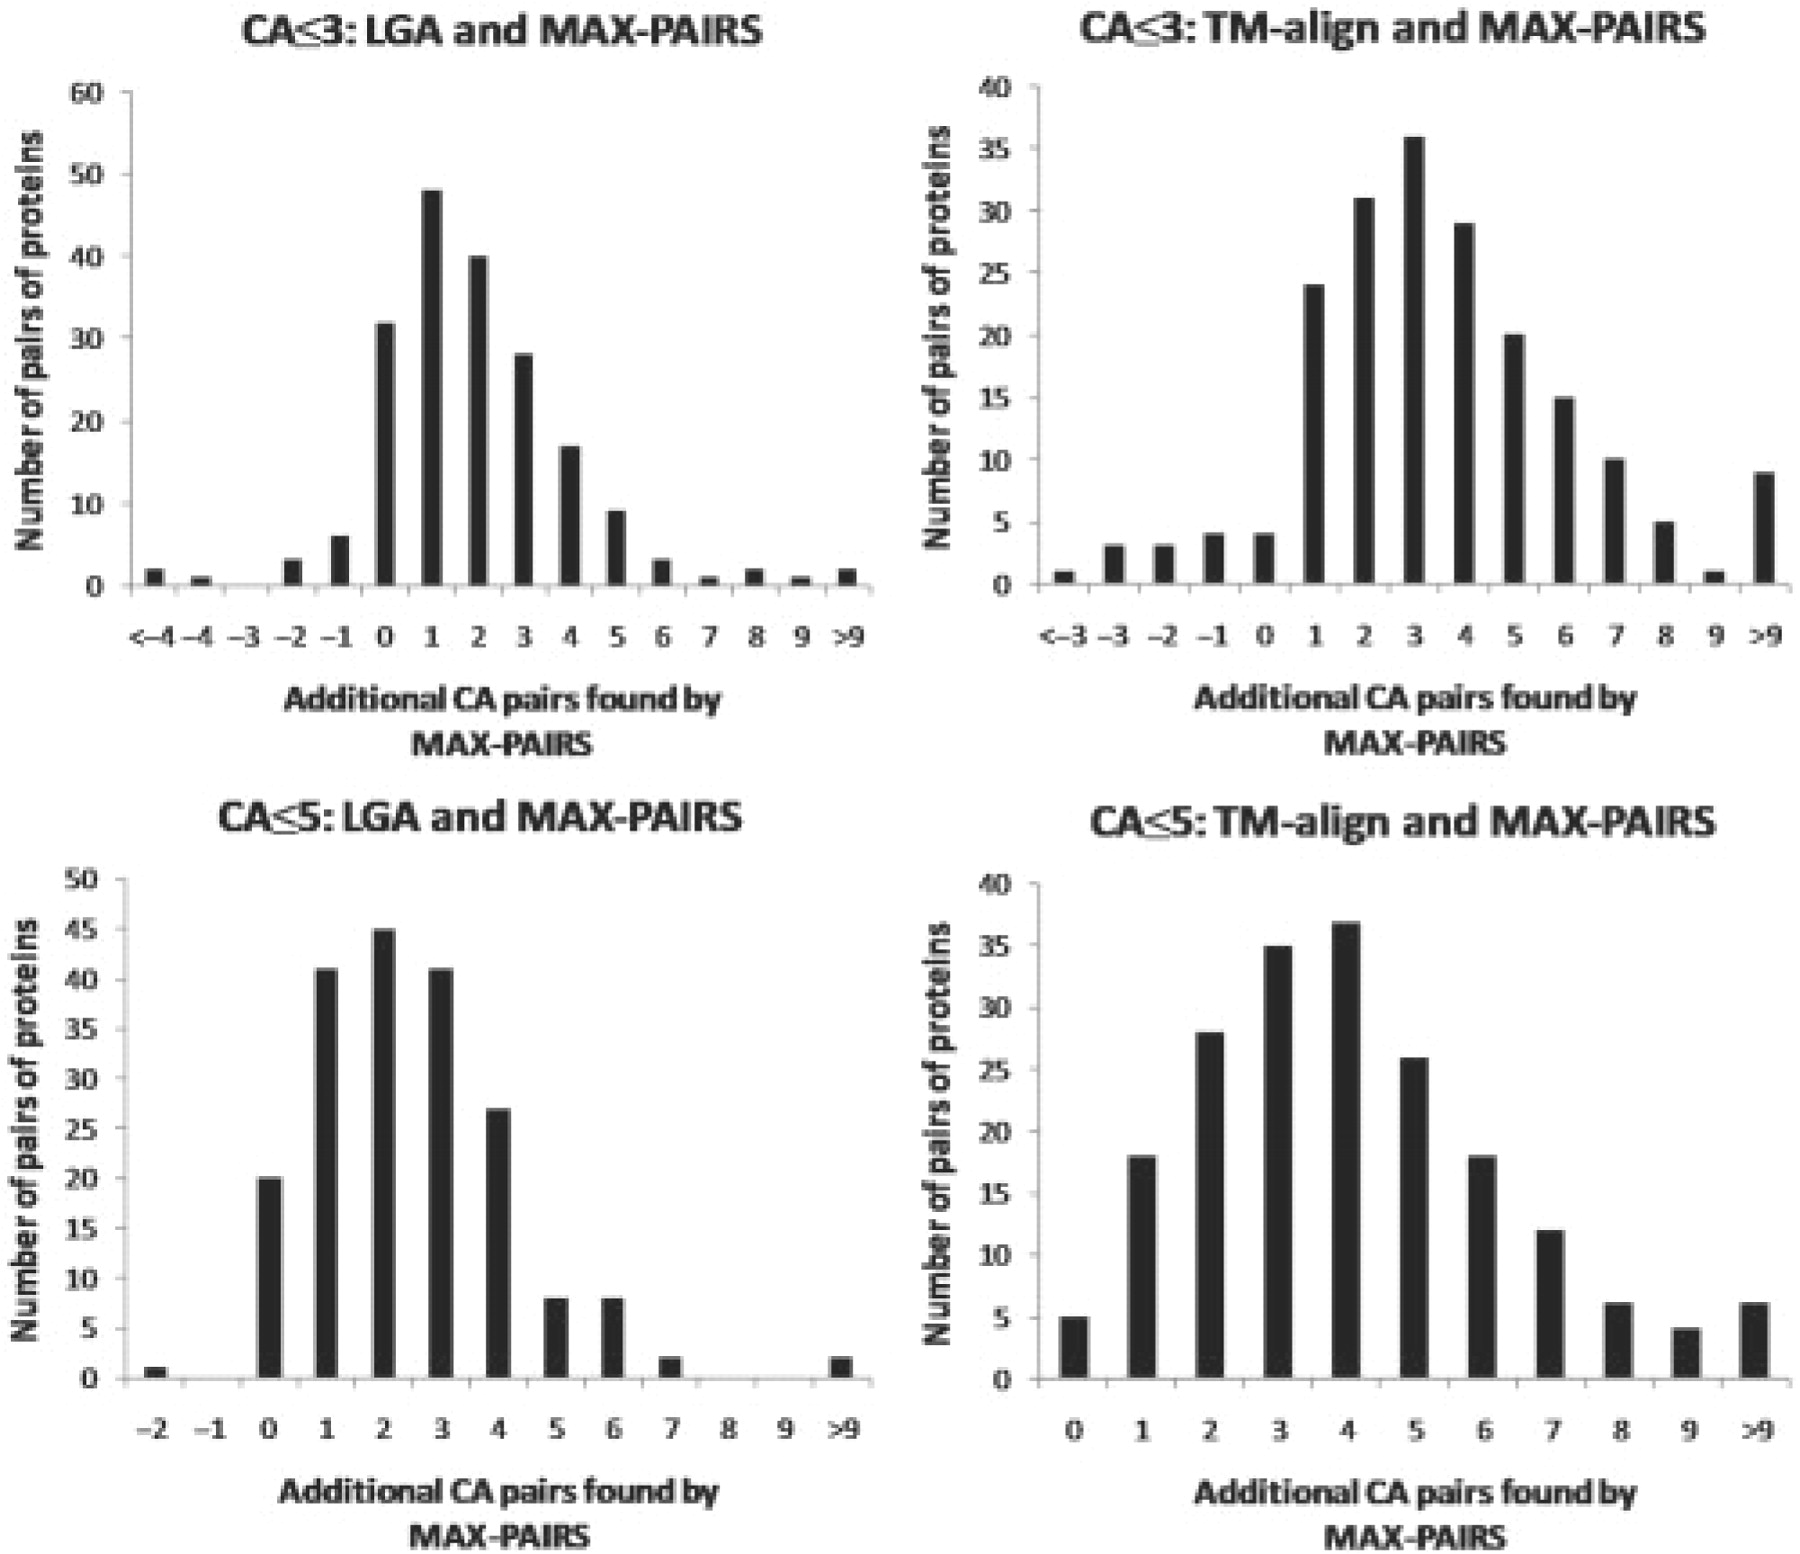
\includegraphics[scale=0.25]{../pictures/btp530f3.jpeg}

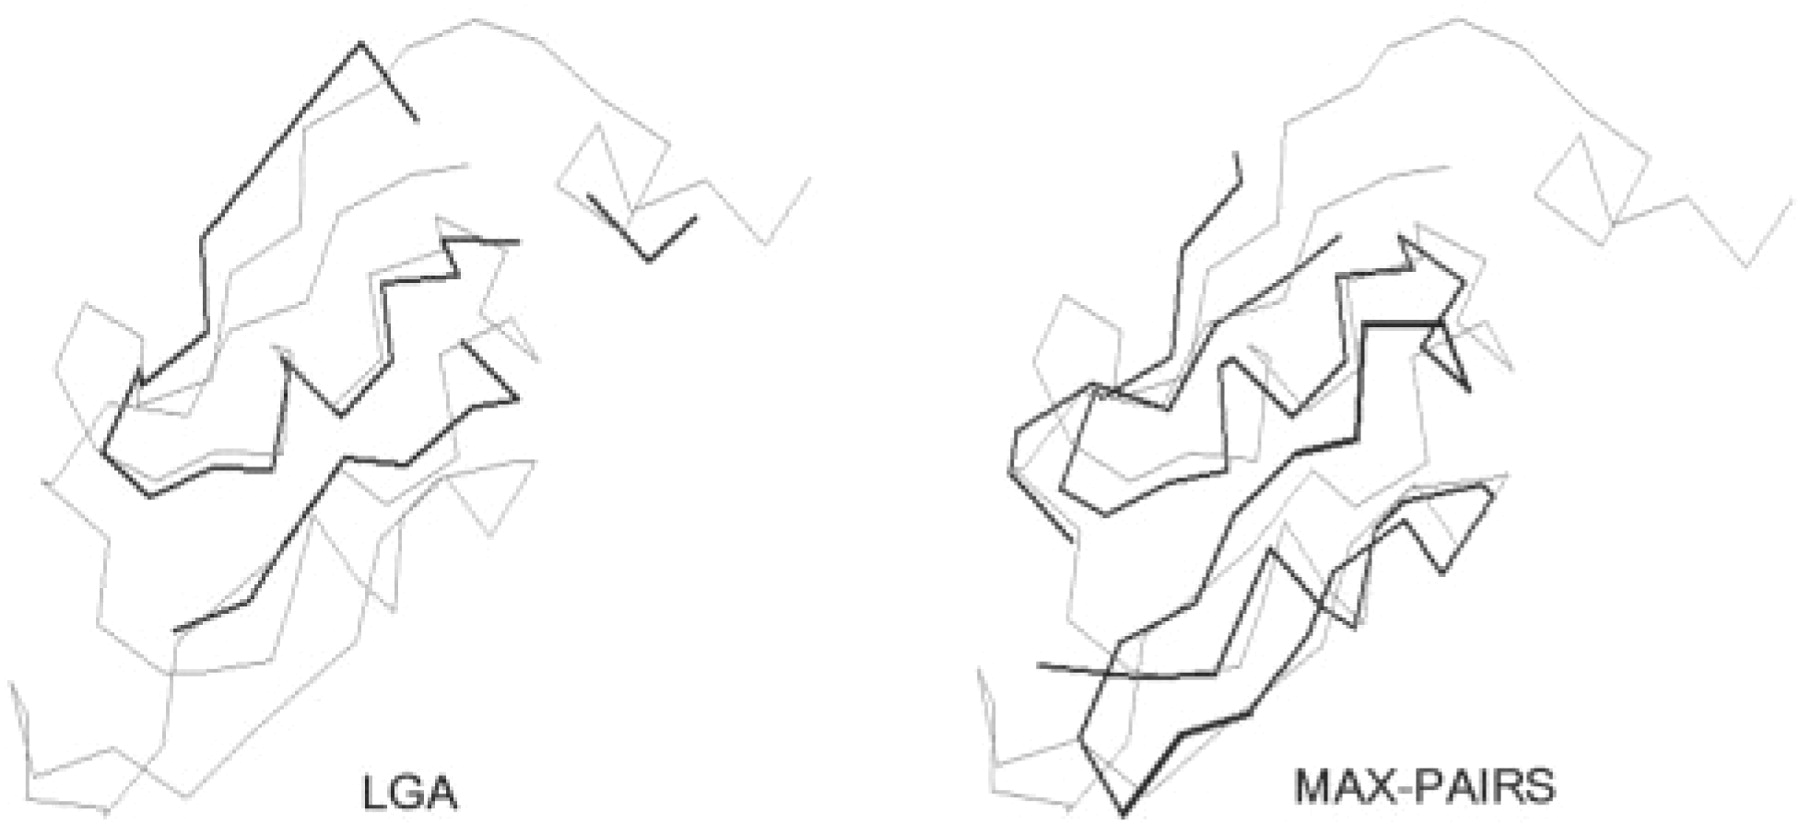
\includegraphics[scale=0.25]{../pictures/btp530f4.jpeg}

В таблице 3 покажем эффективность MAX-PAIRS как функции зависящей от $\eps$ она множестве пар структур из описанного выше датасета. Анализ был произведён на компьюетере с Intel CPU производительностью 2.2 GHz с операционной системой Linux. Результаты собранные в данной таблице предполагают что, хотя LGA и TM-align намного более эффективные программы по сравнению с MAX-PAIRS однако точность MAX-PAIRS превосходит точности этих алгоритмов для всех протестированных значений $\eps$.

\begin{center}
\begin{table}
\caption{ Время работы в зависимости от $\eps$ \angstrom}
\begin{tabular}{|c|c|c|}
\hline
$\eps$ & $CA \leq 3$  & Время работы одной пары (секунд)\\
\hline
1.0 & 11937 & 6608\\
1.5 & 11862 & 713\\
2.0 & 11789 & 140\\
2.5 & 11711 & 46\\
3.0 & 11602 & 19\\
3.5 & 11566 & 9\\
\hline
\end{tabular}
\end{table}
\end{center}
Многие методы попарного структурного выравнивания белков, включая методы, обсуждаемые в этой работе, используют ключевую процедуру для вычисления суперпозиций, которая максимизирует $CA \leq \sigma$ между парой белковых структур. Вполне разумно ожидать, что улучшение этой суперпозиции повышает точность выравнивания структуры белка. Для оценки степени этого улучшения, используется Sisyphus бенчмарк для точности выравнивания Набор тестов Sisyphus содерижт 125 созданных вручную структурных выравниваний для пар белков с нетривиальным структурными отношениями. Эти выравнивания могут быть использованы (как золотые стандарты) для оценки точности метода выравнивания структуры белка. Для того, чтобы сравнить точность выравнивания алгоритмов в данной работе с тончостью методов , ранее протестированных в Sisyphus бенчмарке, использовались только подбножество набора теста Sisyphus содержащего 106 одиночных цепных белков.

Чтобы проверить полезность алгоритмов оптимизации $CA \leq \sigma$, мы модифицировали метод TM-align, заменив исходные суперпозиции TM-align суперпозициями, порождёнными программой MAX-PAIRS. Модифицированная TM-align, названная MP-TM-align, использует TM-align функцию оценивания (TM-score) для вычисления оптимального структурного выравнивания белков совмещённых MAX-PAIRS программой. Как видно из таблицы 4, не только программа MP-TM-align превосходит исходный метод TM-align для каждого сдвига допуска, но и точность этого простого гибридного метода сопоставима с точностью методов проверенных Rocha и коллегами.
\begin{center}
\begin{table}
\caption{ Согласование с эталонными выравниваниями для 6 различных сдвигов}
\begin{tabular}{|c|cccccc|}
\hline
&0&1&2&3&4&5\\
\hline
FLEXPROT&		0.449&	0.672&	0.707&	0.725&	0.742&	0.747\\
MATRAS&			0.776&	0.806&	0.828&	0.836&	0.847&	0.847\\
PD&				0.791&	0.849&	0.858&	0.868&	0.881&	0.882\\
PPM&			0.782& 	0.813& 	0.823&	0.833&	0.843&	0.844\\
RASH&			0.688&	0.793&	0.812&	0.840&	0.854&	0.855\\
SSAP&			0.750&	0.786&	0.797&	0.804&	0.808&	0.811\\
VOROLIGN&		0.722&	0.765&	0.790&	0.808&	0.826&	0.830\\
DALI&			0.800&	0.830&	0.845&	0.851&	0.859&	0.860\\
MATT&			0.829&	0.866&	0.889&	0.904&	0.915&	0.917\\
LGA&			0.765&	0.820&	0.831& 	0.839&	0.847&	0.849\\
TM-align&		0.762&	0.815&	0.823&	0.834&	0.841&	0.844\\
MP-TM-align&	0.809&	0.861&	0.875&	0.884&	0.896&	0.896\\
MP-TM-align+&	0.830&	0.867&	0.881&	0.887&	0.897&	0.898\\
\hline
\end{tabular}
\end{table}
\end{center}
\end{document}